\begin{center}
	\textbf{Feature Maps} \hspace{2em} \textbf{Filters} \\ % Titles for the grids
	\begin{tabular}{c c}
		% First 5x5 grid
		\begin{tabular}{|c|c|c|c|c|}
			\hline
			0 & 1 & 0  & -1 & 1 \\ \hline
			1 & 1 & 0  & -1 & 0 \\ \hline
			1 & 1 & 0  & 0  & 1 \\ \hline
			0 & 0 & 1  & 0  & 1 \\ \hline
			1 & 0 & -1 & -1 & 0 \\ \hline
		\end{tabular}
		 &                      % Separator for the two sets of grids
		% First 3x3 grid
		\begin{tabular}{|c|c|c|}
			\hline
			1 & 0 & -1 \\ \hline
			1 & 0 & -1 \\ \hline
			1 & 0 & -1 \\ \hline
		\end{tabular} \\
		\vspace{2em}            \\ % Adds vertical space between the 5x5 grids
		% Second 5x5 grid
		\begin{tabular}{|c|c|c|c|c|}
			\hline
			1  & 1  & 1  & 0  & 0 \\ \hline
			0  & -1 & 1  & 0  & 0 \\ \hline
			0  & 1  & -1 & -1 & 1 \\ \hline
			-1 & 1  & -1 & 0  & 1 \\ \hline
			1  & 1  & -1 & 0  & 0 \\ \hline
		\end{tabular}
		 &                      % Separator for the two sets of grids
		% Second 3x3 grid (identical to first one in your example)
		\begin{tabular}{|c|c|c|}
			\hline
			1  & 1  & 1  \\ \hline
			0  & 0  & 0  \\ \hline
			-1 & -1 & -1 \\ \hline
		\end{tabular}
	\end{tabular}
\end{center}

In the provided area below, fill in the values resulting from applying a convolutional layer to the input with no zero-padding and a stride of 1. Calculate these numbers before \textbf{any activation function} is applied.
There will be unused cells - place an $\times$ in them. The output you get on the right is the output after \textbf{combining} the results of each channel. Again - there will be unused cells. And don't apply an activation function! (3 pts)

\begin{figure}[H]
	\centering
	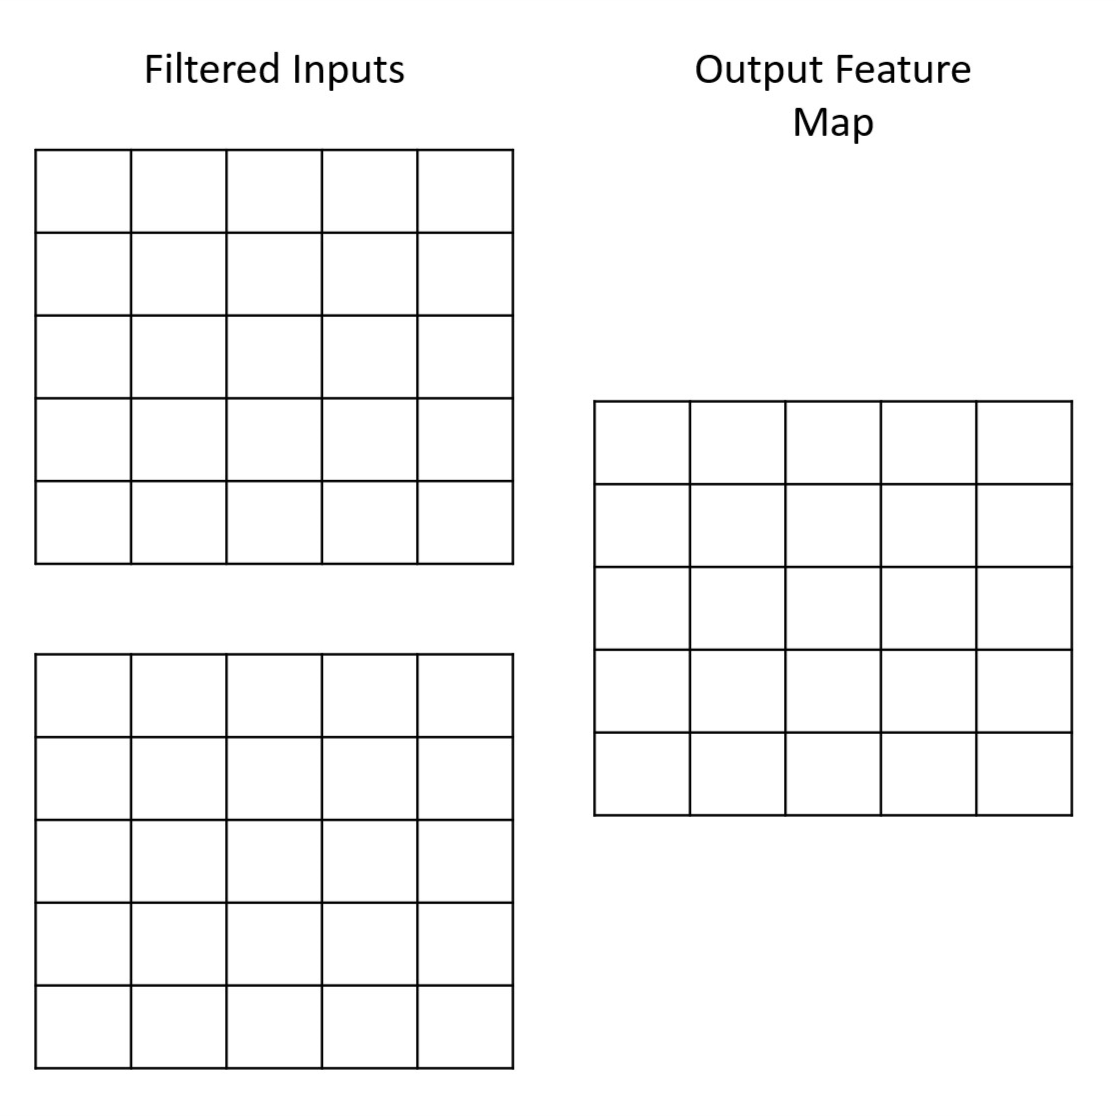
\includegraphics[width=.35\linewidth]{images/conv_question_blanks_1.png}
\end{figure}

\begin{tcolorbox}[title=Solution]
\end{tcolorbox}
